\documentclass[aspectratio=169,11pt]{beamer}
% beamer-theme.tex -- shared look for analysis-deck Beamer decks.
% \input this from Deck.tex (after \documentclass). Everything keys off the seven
% palette colors below: override them for your brand and the whole deck re-tones.
% (The scaffolder can drop a brand palette in via --palette; otherwise this teal/amber
%  default is a clean, neutral civic/analytical look.)

\usepackage[T1]{fontenc}
\usepackage{lmodern}
\usepackage{xcolor}
\usepackage{tikz}
\usepackage{booktabs}
\usepackage{tabularx}
\usepackage{xurl}              % break long URLs at safe characters
\usepackage[htt]{hyphenat}    % allow breaks inside \texttt{} (file paths)
\sloppy
\emergencystretch=3em

% ---- palette (override for brand) ----
\definecolor{deckbg}{HTML}{0E3D49}     % dark-frame background (title / closing)
\definecolor{deckfg}{HTML}{0E7C86}     % primary accent: titles, bars, big numbers
\definecolor{deckfg2}{HTML}{2BB5A0}    % secondary accent
\definecolor{deckhi}{HTML}{E0922B}     % highlight: opportunities / things to notice
\definecolor{deckink}{HTML}{1A2B33}    % body text on light frames
\definecolor{deckmuted}{HTML}{5B7682}  % captions / secondary text
\definecolor{decktint}{HTML}{E8F2F3}   % card / panel fill

\usetheme{default}
\setbeamertemplate{navigation symbols}{}
\setbeamercolor{normal text}{fg=deckink}
\setbeamercolor{frametitle}{fg=deckbg}
\setbeamerfont{frametitle}{series=\bfseries,size=\Large}
\setbeamercolor{itemize item}{fg=deckfg}
\setbeamercolor{itemize subitem}{fg=deckfg2}
\setbeamercolor{itemize/enumerate body}{fg=deckink}
\setbeamertemplate{itemize item}{\textbullet}
\setbeamertemplate{itemize subitem}{\textendash}

% Frame title: bold, colored, and deliberately WITHOUT an underline rule.
% (A horizontal accent rule under the title is a hallmark of AI-generated slides;
%  whitespace separates the title from content just as well.)
\setbeamertemplate{frametitle}{\vskip0.6em\usebeamerfont{frametitle}%
  \usebeamercolor[fg]{frametitle}\insertframetitle\par}

% Optional running footer; comment out for a cleaner look.
% \setbeamertemplate{footline}{\hfill{\tiny\color{deckmuted}\insertshorttitle\quad}\vskip2pt}

% Big-text commands so a slide never carries a raw \fontsize number. This keeps the
% no-hardcoded-numbers linter honest: the only bare numbers left in Deck.tex are layout
% dimensions (which the linter skips), so anything it flags is a real result that belongs
% in a macro. Tune the sizes here once and every slide follows.
\newcommand{\deckeyebrow}[1]{{\small\bfseries #1}}                         % label above a title
\newcommand{\decktitle}[1]{{\fontsize{32}{36}\selectfont\bfseries #1}}     % title-slide title
\newcommand{\deckhead}[1]{{\fontsize{20}{24}\selectfont\bfseries #1}}      % closing / section head
\newcommand{\deckbignum}[2][deckfg]{{\fontsize{26}{30}\selectfont\bfseries\color{#1} #2}}  % standalone stat

% ---- KPI card style (used by deck_helpers.kpi_board) ----
\tikzset{deckcard/.style={rounded corners=5pt, fill=decktint, minimum width=3.9cm,
  minimum height=2.1cm, align=center, inner sep=4pt, text=deckink}}

% ---- dark frame: for title and closing slides ----
% Resets EVERY foreground colour so no element inherits dark-on-dark and vanishes.
% (Beamer's itemize body colour will override a bare \color{white}, so set it here.)
\newenvironment{darkframe}{%
  \setbeamercolor{background canvas}{bg=deckbg}%
  \setbeamercolor{normal text}{fg=white}%
  \setbeamercolor{itemize/enumerate body}{fg=white}%
  \setbeamercolor{itemize/enumerate subbody}{fg=white}%
  \setbeamercolor{itemize item}{fg=deckfg2}%
  \setbeamercolor{itemize subitem}{fg=deckfg2}%
  \begin{frame}\usebeamercolor[fg]{normal text}\color{white}\raggedright}{%
  \end{frame}}
   % palette, frametitle, darkframe, KPI-card style, \decktitle etc.

% Generated numbers -- produced by scripts/generate_deck_assets.py. RUN IT before compiling.
% Every result number on a slide is a macro defined there; never type one into this file.
% (The no-hardcoded-numbers linter enforces this.)
\InputIfFileExists{tables/headlines.tex}{}{}
\providecommand{\PhlHeadline}{\textbf{[run generate\_deck\_assets.py]}}

\title{A Fairer, Revenue-Neutral Path to Property Tax Reform}
\author{}
\date{}

\begin{document}

% ======================================================================
% 1. Title
% ======================================================================
\begin{darkframe}
\vfill
{\color{deckfg2}\deckeyebrow{ PHILADELPHIA LAND VALUE TAX }}\\[1.0em]
\decktitle{ A Fairer, Revenue-Neutral Path to \\ Property Tax Reform }\\[0.5em]
{\large\color{decktint} Land Value Tax: what it does for homeowners, for the city's housing goals, and for the path forward}\\[2.0em]
{\footnotesize\color{deckmuted} Center for Land Economics \quad\textbullet\quad Modeled on Philadelphia's own parcel data}
\vfill
\end{darkframe}

% ======================================================================
% 2. Agenda
% ======================================================================
\begin{frame}{Agenda}
\begin{enumerate}
\item The problem: how Philadelphia taxes today, and what the abatement was trying to fix
\item What Land Value Tax is, and how it improves on the abatement
\item The results: who wins, including Northeast Philadelphia specifically
\item How LVT supports the Mayor's own housing production goals
\item The political and legal path forward
\end{enumerate}
\end{frame}

% ======================================================================
% 3. The problem, part 1 -- land value varies, the tax system doesn't
% ======================================================================
\begin{frame}{Philadelphia taxes buildings the same as land -- but land value isn't uniform}
\begin{columns}[T]
\begin{column}{0.52\linewidth}
\vspace{0.6em}
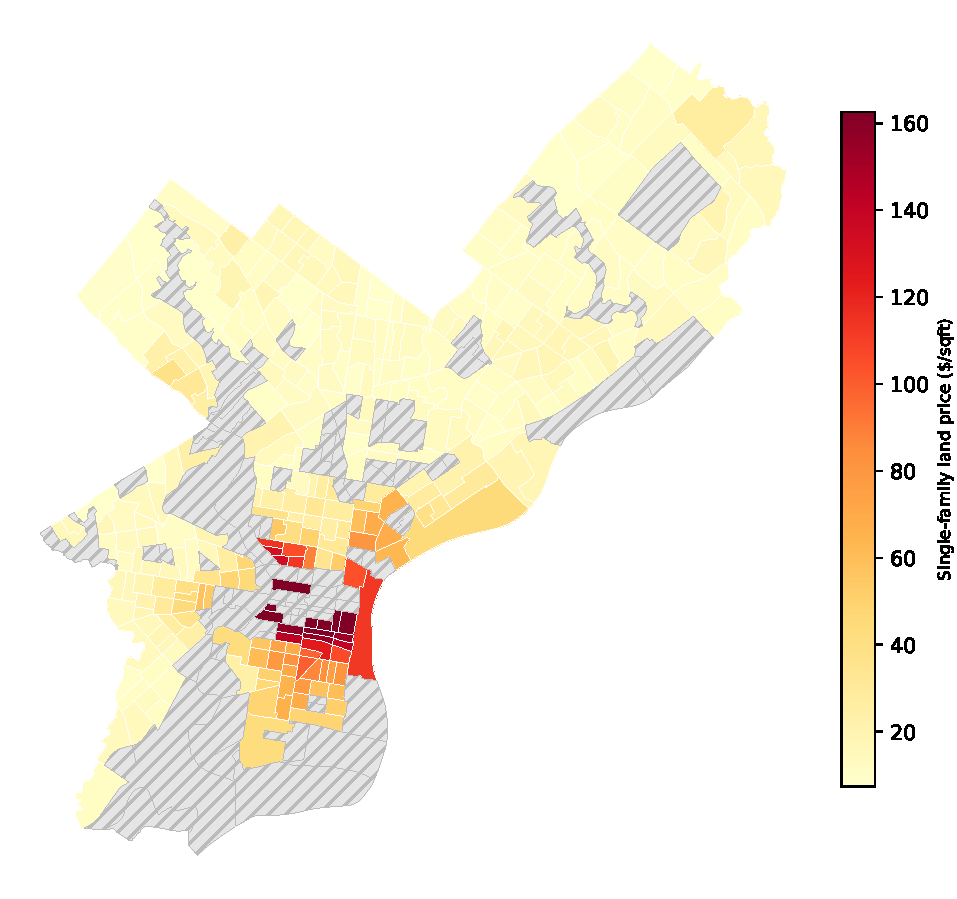
\includegraphics[height=6.4cm]{figures/fhfa_land_price.pdf}
\end{column}
\begin{column}{0.46\linewidth}
\vspace{1.0em}
\begin{itemize}
\item Land value is wildly uneven across the city -- Center City land runs into the hundreds of dollars per square foot; most neighborhoods, a fraction of that
\item Today's property tax hits land and buildings at the identical rate, so it can't tell the difference
\item Result: renovating a home or building new raises your bill just as much as sitting on an empty, well-located lot does nothing to yours
\end{itemize}
\end{column}
\end{columns}
\end{frame}

% ======================================================================
% 4. The problem, part 2 -- the abatement's cliff
% ======================================================================
\begin{frame}{The 10-year abatement papers over the problem -- and creates a new one} % noqa: hardcode
\begin{columns}[T]
\begin{column}{0.5\linewidth}
\vspace{0.6em}
\begin{center}
\deckbignum{\PhlAbatementCliffMedian}\\[0.3em]
{\small\color{deckmuted} median status-quo tax jump when a construction abatement expires, for the \PhlAbatedParcelCount{} Philadelphia parcels currently abated}
\end{center}
\end{column}
\begin{column}{0.5\linewidth}
\vspace{1.0em}
\begin{itemize}
\item Built to encourage building by exempting new construction -- but only new construction, only for ten years, and only from the building tax
\item Real, ongoing cost: Council has cut it back repeatedly since 2019, including a bill Mayor Parker herself introduced as a councilmember, cutting the commercial abatement from 100\% to 90\%  % noqa: hardcode
\item When the clock runs out, the bill jumps all at once -- a cliff for the homeowner, not a phase-in
\end{itemize}
\end{column}
\end{columns}
\end{frame}

% ======================================================================
% 5. What LVT is
% ======================================================================
\begin{frame}{What a Land Value Tax actually does}
\begin{columns}[T]
\begin{column}{0.5\linewidth}
\vspace{0.6em}
\begin{itemize}
\item Splits the property tax into two rates: one for land value, one for building (improvement) value
\item Land gets taxed at a higher rate; buildings get taxed at a lower rate
\item The model here uses a 4:1 split -- land taxed 4 times the rate of buildings
\item Designed to be revenue-neutral: the city collects the same total, just redistributed by what's actually taxed
\end{itemize}
\end{column}
\begin{column}{0.5\linewidth}
\vspace{1.0em}
{\small\color{deckmuted} A simple example}\\[0.4em]
Two identical-value rowhomes, same street:
\begin{itemize}
\item A well-kept home with a nicely finished interior -- its improvement value is high relative to its land, so it pays \emph{less} than it does today
\item A neglected shell on an equally valuable lot -- its land value dominates, so it pays \emph{more} than it does today
\end{itemize}
{\footnotesize\color{deckmuted} Same land, same tax bill either way -- the incentive shifts toward using the land well.}
\end{column}
\end{columns}
\end{frame}

% ======================================================================
% 6. LVT vs. the abatement
% ======================================================================
\begin{frame}{LVT is the abatement, done properly}
\small
\begin{center}
\begin{tabularx}{0.96\linewidth}{@{} X X X @{}}
\toprule
 & \textbf{10-year abatement} & \textbf{Land Value Tax} \\ % noqa: hardcode
\midrule
Who benefits & New construction only & Every property, including existing homeowners \\
How long & 10 years, then a cliff & Permanent \\  % noqa: hardcode
Cost to the city & Foregone revenue -- why Council keeps cutting it back & Revenue-neutral by construction \\
The incentive & Don't tax new buildings & Never tax buildings the same as land \\
\bottomrule
\end{tabularx}
\end{center}
\vspace{0.5em}
\begin{itemize}
\item LVT does what the abatement was trying to do -- don't punish building -- permanently, for every property, paid for by land instead of by revenue the city gives up
\item One honest trade-off: currently-abated parcels move to a full land-value bill, median change \PhlAbatedReformMedian{} -- the newest, most subsidized properties pay closer to their share, while long-time homeowners get relief
\end{itemize}
\end{frame}

% ======================================================================
% 7. Revenue-neutral, verified
% ======================================================================
\begin{frame}{Not a tax cut, not a giveaway -- a swap}
\begin{columns}[T]
\begin{column}{0.5\linewidth}
\vspace{1.2em}
\begin{center}
\deckbignum[deckfg2]{Revenue-neutral}\\[0.3em]
{\small\color{deckmuted} by construction -- modeled gap: \PhlRevenueGapDollars{}, or \PhlRevenueGapPct{} of the levy (rounding, not a real shortfall)}
\end{center}
\end{column}
\begin{column}{0.5\linewidth}
\vspace{1.0em}
\begin{itemize}
\item Every scenario modeled holds total city revenue fixed -- the tax burden moves between properties, not away from the city
\item Independently re-audited: every model notebook was re-executed from scratch and reproduced byte-identical results
\item This is the argument the abatement can't make -- LVT can't be attacked as a giveaway, because nothing is given away
\end{itemize}
\end{column}
\end{columns}
\end{frame}

% ======================================================================
% 8. LVT meets the Mayor's H.O.M.E. plan
% ======================================================================
\begin{frame}{LVT is the tax-policy engine behind the Mayor's own housing goals}
\begin{columns}[T]
\begin{column}{0.5\linewidth}
\vspace{0.6em}
{\small\color{deckmuted} Mayor Parker's H.O.M.E. plan}\\[0.4em]
\begin{itemize}
\item \$2 billion committed to create and preserve 30,000 homes citywide  % noqa: hardcode
\item Built on the same logic LVT applies economy-wide: give tax relief to encourage building, don't penalize it
\end{itemize}
\end{column}
\begin{column}{0.5\linewidth}
\vspace{1.0em}
\begin{itemize}
\item H.O.M.E. does this parcel-by-parcel, program-by-program; LVT does it structurally, for every property in the city, permanently
\item LVT also works the supply side directly -- it makes sitting on vacant, well-located land expensive, not just building on it cheap
\item The two are not competing housing strategies -- LVT is the tax structure that makes the H.O.M.E. plan's logic self-sustaining
\end{itemize}
\end{column}
\end{columns}
\end{frame}

% ======================================================================
% 9. Headline results (decile chart)
% ======================================================================
\begin{frame}{Homeowners win -- and the reform gets fairer once land is priced accurately}
\vspace{0.2em}
{\small\color{deckmuted} Median Single Family Residential tax change, by home value}\\[0.3em]
\begin{columns}[T]
\begin{column}{0.58\linewidth}
\vspace{0.3em}
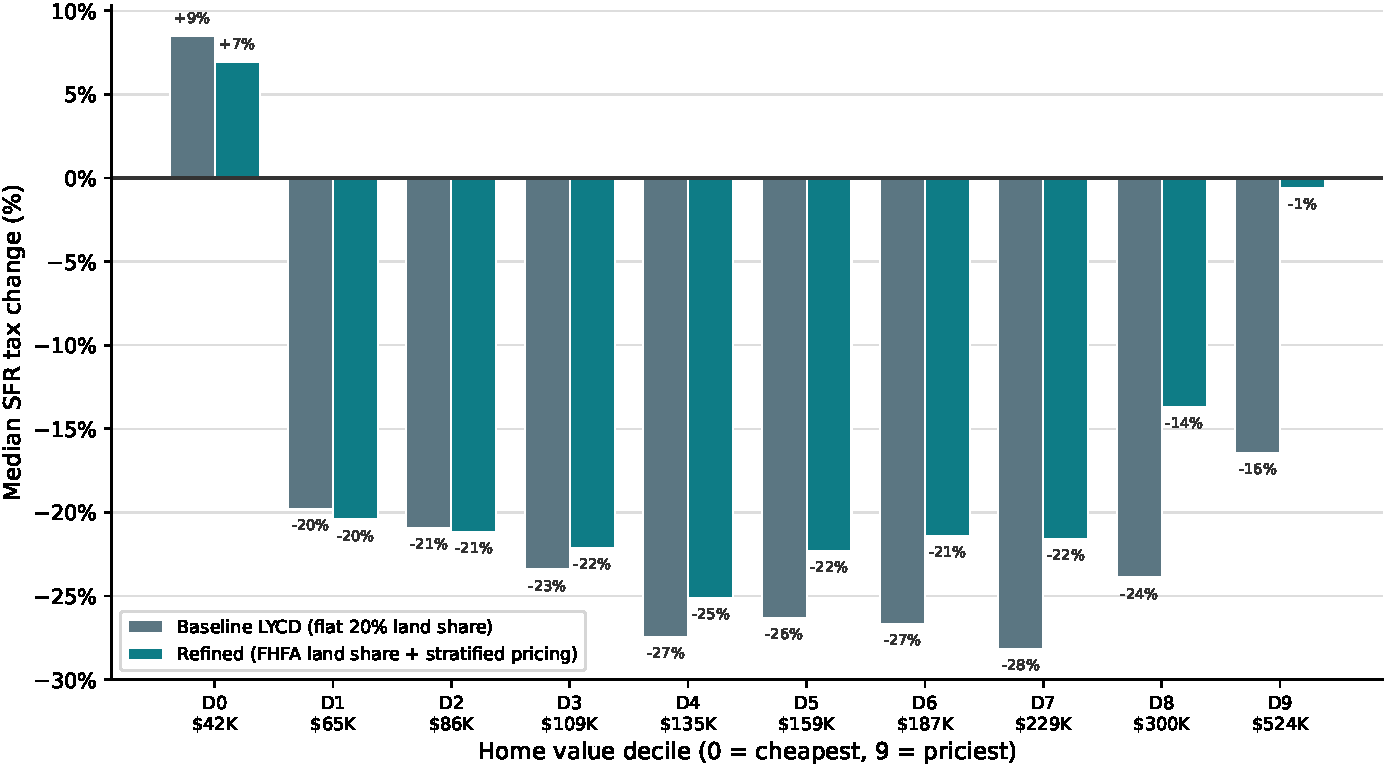
\includegraphics[width=\linewidth]{figures/decile_progressivity.pdf}
\end{column}
\begin{column}{0.4\linewidth}
\vspace{0.1em}
\footnotesize
\begin{itemize}
\item \PhlSfrWinRateRefined{} of Philadelphia homeowners see a tax cut citywide -- median change \PhlSfrMedianRefined{}
\item Modest homes (around \PhlDecileBottomValue{}) are essentially untouched: \PhlDecileBottomRefined{}
\item The priciest homes (around \PhlDecileTopValue{}) lose most of an oversized cut, from \PhlDecileTopBaseline{} down to \PhlDecileTopRefined{} -- they were only getting it because their land was underpriced
\item Fairness story: the reform gets \emph{more} progressive once land values reflect real neighborhood demand
\end{itemize}
\end{column}
\end{columns}
\end{frame}

% ======================================================================
% 10. Northeast Philadelphia, honestly
% ======================================================================
\begin{frame}{Northeast Philadelphia: a smaller win, honestly stated -- and it holds up}
\begin{columns}[T]
\begin{column}{0.55\linewidth}
\vspace{0.6em}
\begin{tabularx}{\linewidth}{@{} Xrr @{}}
\toprule
District & Baseline LYCD & Refined LYCD \\
\midrule
District 6 (Lower NE) & -22.1\% & -21.4\% \\
District 9 (Near NE) & -17.9\% & -19.7\% \\
District 10 (Far NE) & -21.6\% & -15.5\% \\
\bottomrule
\end{tabularx}

\vspace{0.8em}
{\footnotesize\color{deckmuted} Median SFR tax change by council district. Citywide median: \PhlCitywideDistrictMedianRefined{}.}
\end{column}
\begin{column}{0.42\linewidth}
\vspace{0.5em}
\small
\begin{itemize}
\item The median Northeast homeowner still gets a tax cut in every district and every land-valuation method tested -- smaller than the citywide median, but real
\item With more accurate, neighborhood-specific land values (right column), District 9 actually improves and District 6 barely moves
\item Not ``no effect,'' but ``a real, if smaller, win that gets better with better data''
\end{itemize}
\end{column}
\end{columns}
\end{frame}

% ======================================================================
% 11. Vacant land / blight
% ======================================================================
\begin{frame}{The sharpest incentive change: vacant and blighted land}
\begin{columns}[T]
\begin{column}{0.45\linewidth}
\vspace{1.2em}
\begin{center}
\deckbignum[deckhi]{\PhlVacantLandMedianRefined{}}\\[0.3em]
{\small\color{deckmuted} median tax change for vacant land, citywide}
\end{center}
\end{column}
\begin{column}{0.5\linewidth}
\vspace{1.0em}
\begin{itemize}
\item Every other category's cut or increase is modest by comparison -- vacant land is where the reform bites hardest, exactly as intended
\item Directly supports the H.O.M.E. plan's production goal: it becomes expensive to sit on a buildable lot, not just cheap to build on one
\item This is also the strongest-polling public frame for the reform -- lead with blight, not with the mechanics of land valuation
\end{itemize}
\end{column}
\end{columns}
\end{frame}

% ======================================================================
% 12. Citywide political coalition alignment (GENERIC -- no names)
% ======================================================================
\begin{frame}{The reform doesn't put any elected official's own base at odds with their vote}
\begin{itemize}
\item Across the city's political geography -- district and at-large officials alike -- electoral strongholds are not disproportionately exposed to losses under the reform
\item Where homeowners in any official's base do see an increase, the losses are shallow -- nowhere close to the losses concentrated elsewhere
\item The largest dollar increases fall overwhelmingly on vacant-land holders, not on homeowners in any particular official's coalition
\item In plain terms: this is not a reform that asks any officeholder to choose between good policy and their own re-election
\end{itemize}
\vspace{1.0em}
{\footnotesize\color{deckmuted} Independently audited across multiple land-valuation methods; see appendix for methodology.}
\end{frame}

% ======================================================================
% 13. Legal pathway
% ======================================================================
\begin{frame}{The path runs through Harrisburg, not just City Hall}
\begin{columns}[T]
\begin{column}{0.5\linewidth}
\vspace{0.6em}
\begin{itemize}
\item Pennsylvania's Uniformity Clause means Philadelphia needs state enabling legislation before City Council can act -- this is not a City Council vote alone
\end{itemize}
\end{column}
\begin{column}{0.48\linewidth}
\vspace{0.6em}
{\small\color{deckmuted} Active relationships, not cold outreach}\\[0.4em]
\begin{itemize}
\item \textbf{PA House:} Reps. Hohenstein and Khan have both expressed interest -- Khan is especially well suited given his pro-housing legislative record and his severance tax bill
\item \textbf{PA Senate:} Sen. Saval is a natural fit
\item We are already in direct contact with Hohenstein and Khan
\end{itemize}
\end{column}
\end{columns}
\end{frame}

% ======================================================================
% 14. Coalition landscape
% ======================================================================
\begin{frame}{Where the coalition stands today}
\begin{center}
\begin{tabularx}{0.96\linewidth}{@{} X X @{}}
\toprule
\textbf{For} & \textbf{Against} \\
\midrule
Philly YIMBY / 5th Square (zoning and infill advocacy infrastructure); nonpartisan technical LVT advocates; renters (roughly half of Philadelphia households) and younger voters as a large, if still unorganized, latent constituency &
No organization has taken a public anti-LVT position in Philadelphia specifically -- the clearest identifiable opposition is a small, concentrated group of large vacant-land owners with a direct financial stake \\
\bottomrule
\end{tabularx}
\end{center}
\vspace{0.8em}
\begin{itemize}
\item No sitting Philadelphia official has taken an affirmative public position on LVT specifically -- this is a genuinely open field, not a fight against entrenched opposition
\item The gap is coalition-formation, not resistance
\end{itemize}
\end{frame}

% ======================================================================
% 15. Recommended next steps
% ======================================================================
\begin{frame}{What moving forward actually looks like}
\begin{enumerate}
\item \textbf{Near term:} brief Hohenstein and Khan's offices on the modeled results; identify a prime co-sponsor pairing for state enabling legislation
\item \textbf{Parallel track:} bring these results to the Mayor's office, framed against the H.O.M.E. plan's own goals
\item \textbf{Medium term:} formalize the coalition -- YIMBY/5th Square, renter organizations, and any interested labor partners -- around a specific legislative ask
\item \textbf{Ongoing:} keep refining the underlying land-value data (this deck already reflects one such refinement) so the modeling only gets more defensible over time
\end{enumerate}
\end{frame}

% ======================================================================
% 16. Closing
% ======================================================================
\begin{darkframe}
\deckeyebrow{ PHILADELPHIA LAND VALUE TAX }\\[1.0em]
\deckhead{A reform that pays for itself, and pays off for homeowners}\\[1.2em]
\begin{itemize}
\item \PhlSfrWinRateRefined{} of homeowners see a tax cut -- revenue-neutral, verified
\item Fairer than the abatement it would replace, and structurally aligned with the Mayor's own housing production goals
\item An open political field -- no entrenched opposition, real relationships already underway in Harrisburg
\end{itemize}
\vfill
{\footnotesize\color{deckmuted} Center for Land Economics \quad\textbullet\quad Full methodology in appendix}
\end{darkframe}

% ======================================================================
% APPENDIX
% ======================================================================
\begin{darkframe}
\deckhead{Appendix}\\[0.6em]
{\small\color{decktint} Methodology, full district results, and sources}
\end{darkframe}

\begin{frame}{A1 -- Methodology: three ways to estimate land value}
\begin{itemize}
\item \textbf{OPA (city assessor):} the city's own raw land/building split -- a large share of parcels default to a flat, administratively simplified split rather than a true appraisal
\item \textbf{LYCD (baseline model):} a zone-median approach built from the city's own micro-geographic assessment zones, using a flat 20\% land-share assumption for improved parcels % noqa: hardcode
\item \textbf{FHFA-refined (this deck's headline numbers):} replaces the flat 20\% assumption with neighborhood-specific land shares from an independent federal (FHFA) land-price dataset, and separates residential from commercial/industrial zone pricing % noqa: hardcode
\end{itemize}
\vspace{0.6em}
{\footnotesize\color{deckmuted} All three are modeled from Philadelphia's own public parcel data; results in this deck use the refined method unless noted as ``baseline.''}
\end{frame}

\begin{frame}{A2 -- Full council district results}
\begin{tabularx}{\linewidth}{@{} Xrr @{}}
\toprule
District & Baseline LYCD (median SFR) & Refined LYCD (median SFR) \\
\midrule
District 1 & -21.3\% & -7.2\% \\
District 2 & -24.9\% & -13.3\% \\
District 3 & -27.5\% & -25.0\% \\
District 4 & -23.9\% & -19.4\% \\
District 5 & -21.9\% & -12.8\% \\
District 6 & -22.1\% & -21.4\% \\
District 7 & -28.1\% & -28.1\% \\
District 8 & -24.2\% & -23.9\% \\
District 9 & -17.9\% & -19.7\% \\
District 10 & -21.6\% & -15.5\% \\
\bottomrule
\end{tabularx}

\vspace{0.6em}
{\footnotesize\color{deckmuted} Median Single Family Residential tax change by council district, baseline vs. refined land-valuation method.}
\end{frame}

\begin{frame}{A3 -- Revenue neutrality and audit methodology}
\begin{itemize}
\item Every scenario is solved to hold total modeled revenue fixed by construction (the split-rate solver targets the city's actual current revenue)
\item All four core model variants were independently re-executed from source notebooks and reproduced byte-identical results
\item The refined land-valuation method was itself stress-tested: a full assumption/logic/implementation audit is on file, covering data provenance, model sensitivity to the split ratio and land-share assumptions, and the political-exposure findings
\end{itemize}
\end{frame}

\begin{frame}{A4 -- Sources}
\begin{itemize}
\item Philadelphia Office of Property Assessment (OPA) parcel and assessment data
\item Federal Housing Finance Agency, land-price and land-share dataset (Davis, Larson, Oliner \& Shui)
\item City of Philadelphia, H.O.M.E. housing plan announcement (March 2025)
\item Philadelphia City Council legislative record (abatement reform history)
\end{itemize}
\end{frame}

\end{document}
